% Options for packages loaded elsewhere
\PassOptionsToPackage{unicode}{hyperref}
\PassOptionsToPackage{hyphens}{url}
\PassOptionsToPackage{dvipsnames,svgnames,x11names}{xcolor}
%
\documentclass[
  letterpaper,
  DIV=11,
  numbers=noendperiod]{scrartcl}

\usepackage{amsmath,amssymb}
\usepackage{lmodern}
\usepackage{iftex}
\ifPDFTeX
  \usepackage[T1]{fontenc}
  \usepackage[utf8]{inputenc}
  \usepackage{textcomp} % provide euro and other symbols
\else % if luatex or xetex
  \usepackage{unicode-math}
  \defaultfontfeatures{Scale=MatchLowercase}
  \defaultfontfeatures[\rmfamily]{Ligatures=TeX,Scale=1}
\fi
% Use upquote if available, for straight quotes in verbatim environments
\IfFileExists{upquote.sty}{\usepackage{upquote}}{}
\IfFileExists{microtype.sty}{% use microtype if available
  \usepackage[]{microtype}
  \UseMicrotypeSet[protrusion]{basicmath} % disable protrusion for tt fonts
}{}
\makeatletter
\@ifundefined{KOMAClassName}{% if non-KOMA class
  \IfFileExists{parskip.sty}{%
    \usepackage{parskip}
  }{% else
    \setlength{\parindent}{0pt}
    \setlength{\parskip}{6pt plus 2pt minus 1pt}}
}{% if KOMA class
  \KOMAoptions{parskip=half}}
\makeatother
\usepackage{xcolor}
\setlength{\emergencystretch}{3em} % prevent overfull lines
\setcounter{secnumdepth}{-\maxdimen} % remove section numbering
% Make \paragraph and \subparagraph free-standing
\ifx\paragraph\undefined\else
  \let\oldparagraph\paragraph
  \renewcommand{\paragraph}[1]{\oldparagraph{#1}\mbox{}}
\fi
\ifx\subparagraph\undefined\else
  \let\oldsubparagraph\subparagraph
  \renewcommand{\subparagraph}[1]{\oldsubparagraph{#1}\mbox{}}
\fi

\usepackage{color}
\usepackage{fancyvrb}
\newcommand{\VerbBar}{|}
\newcommand{\VERB}{\Verb[commandchars=\\\{\}]}
\DefineVerbatimEnvironment{Highlighting}{Verbatim}{commandchars=\\\{\}}
% Add ',fontsize=\small' for more characters per line
\newenvironment{Shaded}{}{}
\newcommand{\AlertTok}[1]{\textcolor[rgb]{0.16,0.16,0.16}{\textbf{\colorbox[rgb]{0.80,0.14,0.11}{#1}}}}
\newcommand{\AnnotationTok}[1]{\textcolor[rgb]{0.60,0.59,0.10}{#1}}
\newcommand{\AttributeTok}[1]{\textcolor[rgb]{0.84,0.60,0.13}{#1}}
\newcommand{\BaseNTok}[1]{\textcolor[rgb]{0.96,0.45,0.00}{#1}}
\newcommand{\BuiltInTok}[1]{\textcolor[rgb]{0.84,0.36,0.05}{#1}}
\newcommand{\CharTok}[1]{\textcolor[rgb]{0.69,0.38,0.53}{#1}}
\newcommand{\CommentTok}[1]{\textcolor[rgb]{0.57,0.51,0.45}{#1}}
\newcommand{\CommentVarTok}[1]{\textcolor[rgb]{0.57,0.51,0.45}{#1}}
\newcommand{\ConstantTok}[1]{\textcolor[rgb]{0.69,0.38,0.53}{\textbf{#1}}}
\newcommand{\ControlFlowTok}[1]{\textcolor[rgb]{0.80,0.14,0.11}{\textbf{#1}}}
\newcommand{\DataTypeTok}[1]{\textcolor[rgb]{0.84,0.60,0.13}{#1}}
\newcommand{\DecValTok}[1]{\textcolor[rgb]{0.96,0.45,0.00}{#1}}
\newcommand{\DocumentationTok}[1]{\textcolor[rgb]{0.60,0.59,0.10}{#1}}
\newcommand{\ErrorTok}[1]{\textcolor[rgb]{0.80,0.14,0.11}{\underline{#1}}}
\newcommand{\ExtensionTok}[1]{\textcolor[rgb]{0.41,0.62,0.42}{\textbf{#1}}}
\newcommand{\FloatTok}[1]{\textcolor[rgb]{0.96,0.45,0.00}{#1}}
\newcommand{\FunctionTok}[1]{\textcolor[rgb]{0.41,0.62,0.42}{#1}}
\newcommand{\ImportTok}[1]{\textcolor[rgb]{0.41,0.62,0.42}{#1}}
\newcommand{\InformationTok}[1]{\textcolor[rgb]{0.16,0.16,0.16}{\colorbox[rgb]{0.51,0.65,0.60}{#1}}}
\newcommand{\KeywordTok}[1]{\textcolor[rgb]{0.24,0.22,0.21}{\textbf{#1}}}
\newcommand{\NormalTok}[1]{\textcolor[rgb]{0.24,0.22,0.21}{#1}}
\newcommand{\OperatorTok}[1]{\textcolor[rgb]{0.24,0.22,0.21}{#1}}
\newcommand{\OtherTok}[1]{\textcolor[rgb]{0.41,0.62,0.42}{#1}}
\newcommand{\PreprocessorTok}[1]{\textcolor[rgb]{0.84,0.36,0.05}{#1}}
\newcommand{\RegionMarkerTok}[1]{\textcolor[rgb]{0.57,0.51,0.45}{\colorbox[rgb]{0.98,0.96,0.84}{#1}}}
\newcommand{\SpecialCharTok}[1]{\textcolor[rgb]{0.69,0.38,0.53}{#1}}
\newcommand{\SpecialStringTok}[1]{\textcolor[rgb]{0.60,0.59,0.10}{#1}}
\newcommand{\StringTok}[1]{\textcolor[rgb]{0.60,0.59,0.10}{#1}}
\newcommand{\VariableTok}[1]{\textcolor[rgb]{0.27,0.52,0.53}{#1}}
\newcommand{\VerbatimStringTok}[1]{\textcolor[rgb]{0.60,0.59,0.10}{#1}}
\newcommand{\WarningTok}[1]{\textcolor[rgb]{0.16,0.16,0.16}{\colorbox[rgb]{0.98,0.74,0.18}{#1}}}

\providecommand{\tightlist}{%
  \setlength{\itemsep}{0pt}\setlength{\parskip}{0pt}}\usepackage{longtable,booktabs,array}
\usepackage{calc} % for calculating minipage widths
% Correct order of tables after \paragraph or \subparagraph
\usepackage{etoolbox}
\makeatletter
\patchcmd\longtable{\par}{\if@noskipsec\mbox{}\fi\par}{}{}
\makeatother
% Allow footnotes in longtable head/foot
\IfFileExists{footnotehyper.sty}{\usepackage{footnotehyper}}{\usepackage{footnote}}
\makesavenoteenv{longtable}
\usepackage{graphicx}
\makeatletter
\def\maxwidth{\ifdim\Gin@nat@width>\linewidth\linewidth\else\Gin@nat@width\fi}
\def\maxheight{\ifdim\Gin@nat@height>\textheight\textheight\else\Gin@nat@height\fi}
\makeatother
% Scale images if necessary, so that they will not overflow the page
% margins by default, and it is still possible to overwrite the defaults
% using explicit options in \includegraphics[width, height, ...]{}
\setkeys{Gin}{width=\maxwidth,height=\maxheight,keepaspectratio}
% Set default figure placement to htbp
\makeatletter
\def\fps@figure{htbp}
\makeatother

% load packages
\usepackage{geometry}
\usepackage{xcolor}
\usepackage{eso-pic}
\usepackage{fancyhdr}
\usepackage{sectsty}
\usepackage{fontspec}
\usepackage{titlesec}
\usepackage{listings} % For code listings

%% Set page size with a wider right margin
\geometry{a4paper, total={170mm,257mm}, left=20mm, top=20mm, bottom=20mm, right=50mm}

%% Define colors
\definecolor{light}{HTML}{D73F09}
\definecolor{highlight}{HTML}{800080}
\definecolor{dark}{HTML}{330033}

%% Let's add the border on the right hand side 
\AddToShipoutPicture{% 
    \AtPageLowerLeft{% 
        \put(\LenToUnit{\dimexpr\paperwidth-3cm},0){% 
            \color{light}\rule{3cm}{\LenToUnit\paperheight}%
          }%
     }%
     % logo
    \AtPageLowerLeft{% start the bar at the bottom right of the page
        \put(\LenToUnit{\dimexpr\paperwidth-3.95cm},26cm){% move it to the top right
            \color{light}
\includegraphics[width=5cm]{_extensions/nrennie/PrettyPDF/logo.png}
          }%
     }%
}

%% Style the page number
\fancypagestyle{mystyle}{
  \fancyhf{}
  \renewcommand\headrulewidth{0pt}
  \fancyfoot[R]{\fontsize{28}{12}\selectfont\thepage} % Increase the font size by 10pt
  \fancyfootoffset{3.65cm}
}
\setlength{\footskip}{20pt}

%% style the chapter/section fonts
\chapterfont{\color{dark}\fontsize{20}{16.8}\selectfont}
\sectionfont{\color{dark}\fontsize{20}{16.8}\selectfont}
\subsectionfont{\color{dark}\fontsize{14}{16.8}\selectfont}
\titleformat{\subsection}
  {\sffamily\Large\bfseries}{\thesection}{1em}{}[{\titlerule[0.8pt]}]
  
% left align title
\makeatletter
\renewcommand{\maketitle}{\bgroup\setlength{\parindent}{0pt}
\begin{flushleft}
  {\sffamily\huge\textbf{\MakeUppercase{\@title}}} \vspace{0.3cm} \newline
  {\Large {\@subtitle}} \newline
  {\large\@author} \newline
  {\large\today} % Include the full date here
\end{flushleft}\egroup
}
\makeatother


%% Use some custom fonts
\setsansfont{Georgia}[
    Path=_extensions/nrennie/PrettyPDF/Georgia/,
    Scale=0.9,
    Extension = .ttf,
    UprightFont=*,
    BoldFont=*b,
    ItalicFont=*i,
    ]

\setmainfont{Kievit}[
    Path=_extensions/nrennie/PrettyPDF/Kievit/,
    Scale=0.9,
    Extension = .ttf,
    UprightFont=* Regular,
    BoldFont=* Bold,
    ItalicFont=* Black Italic,
    ]
\KOMAoption{captions}{tableheading}
\makeatletter
\makeatother
\makeatletter
\makeatother
\makeatletter
\@ifpackageloaded{caption}{}{\usepackage{caption}}
\AtBeginDocument{%
\ifdefined\contentsname
  \renewcommand*\contentsname{Table of contents}
\else
  \newcommand\contentsname{Table of contents}
\fi
\ifdefined\listfigurename
  \renewcommand*\listfigurename{List of Figures}
\else
  \newcommand\listfigurename{List of Figures}
\fi
\ifdefined\listtablename
  \renewcommand*\listtablename{List of Tables}
\else
  \newcommand\listtablename{List of Tables}
\fi
\ifdefined\figurename
  \renewcommand*\figurename{Figure}
\else
  \newcommand\figurename{Figure}
\fi
\ifdefined\tablename
  \renewcommand*\tablename{Table}
\else
  \newcommand\tablename{Table}
\fi
}
\@ifpackageloaded{float}{}{\usepackage{float}}
\floatstyle{ruled}
\@ifundefined{c@chapter}{\newfloat{codelisting}{h}{lop}}{\newfloat{codelisting}{h}{lop}[chapter]}
\floatname{codelisting}{Listing}
\newcommand*\listoflistings{\listof{codelisting}{List of Listings}}
\makeatother
\makeatletter
\@ifpackageloaded{caption}{}{\usepackage{caption}}
\@ifpackageloaded{subcaption}{}{\usepackage{subcaption}}
\makeatother
\makeatletter
\@ifpackageloaded{tcolorbox}{}{\usepackage[many]{tcolorbox}}
\makeatother
\makeatletter
\@ifundefined{shadecolor}{\definecolor{shadecolor}{HTML}{000000}}
\makeatother
\makeatletter
\makeatother
\ifLuaTeX
  \usepackage{selnolig}  % disable illegal ligatures
\fi
\IfFileExists{bookmark.sty}{\usepackage{bookmark}}{\usepackage{hyperref}}
\IfFileExists{xurl.sty}{\usepackage{xurl}}{} % add URL line breaks if available
\urlstyle{same} % disable monospaced font for URLs
\hypersetup{
  pdftitle={ST557: Homework 1},
  pdfauthor={Brian Cervantes Alvarez},
  colorlinks=true,
  linkcolor={highlight},
  filecolor={Maroon},
  citecolor={Blue},
  urlcolor={highlight},
  pdfcreator={LaTeX via pandoc}}

\title{ST557: Homework 1}
\author{Brian Cervantes Alvarez}
\date{10/6/23}

\begin{document}
\maketitle
\pagestyle{mystyle}

\ifdefined\Shaded\renewenvironment{Shaded}{\begin{tcolorbox}[breakable, interior hidden, enhanced, boxrule=0pt, borderline west={3pt}{0pt}{shadecolor}, frame hidden, sharp corners]}{\end{tcolorbox}}\fi

\hypertarget{question-1}{%
\section{Question 1}\label{question-1}}

\begin{Shaded}
\begin{Highlighting}[]
\CommentTok{\# Set random seed for reproducibility}
\FunctionTok{set.seed}\NormalTok{(}\DecValTok{503}\NormalTok{)}

\CommentTok{\# Read HW1Q1 dataset in using base R}
\NormalTok{ds }\OtherTok{\textless{}{-}} \FunctionTok{read.csv}\NormalTok{(}\StringTok{"HW1Q1.csv"}\NormalTok{)}
\CommentTok{\# Show first 5 rows}
\FunctionTok{print}\NormalTok{(}\FunctionTok{head}\NormalTok{(ds,}\DecValTok{50}\NormalTok{))}
\end{Highlighting}
\end{Shaded}

\begin{verbatim}
       X     Y
1  -1.54  0.46
2  -4.25 -1.23
3  -0.85  0.34
4  -2.90 -0.94
5  -1.09 -0.84
6  -5.92 -0.70
7   3.51  2.92
8   0.09  0.76
9  -2.08 -0.99
10  5.01  1.58
11  3.22 -0.43
12  3.67  1.29
13 -1.61 -1.60
14  2.23  1.90
15  0.20 -0.06
16  4.39  1.50
17  1.15 -1.81
18  3.63  0.99
19 -4.32 -0.72
20  1.42  0.82
\end{verbatim}

\newpage{}

\hypertarget{part-a}{%
\subsection{Part A}\label{part-a}}

Read this data into R using read.csv(). Create a 2-dimensional scatter
plot of the 20 observations (use plot() function in R).

\begin{Shaded}
\begin{Highlighting}[]
\CommentTok{\# Get X and Y Components into vectors}
\NormalTok{x }\OtherTok{=}\NormalTok{ ds}\SpecialCharTok{$}\NormalTok{X}
\NormalTok{y }\OtherTok{=}\NormalTok{ ds}\SpecialCharTok{$}\NormalTok{Y}

\CommentTok{\# Create scatter plot of Y \textasciitilde{} X}
\FunctionTok{plot}\NormalTok{(x,y)}
\end{Highlighting}
\end{Shaded}

\begin{figure}[H]

{\centering 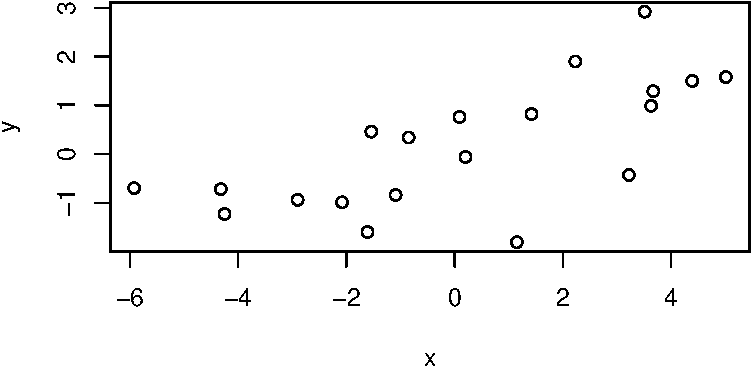
\includegraphics{CervantesAlvarez_Brian_HW1_ST557_files/figure-pdf/unnamed-chunk-2-1.pdf}

}

\end{figure}

\newpage{}

\hypertarget{part-b}{%
\subsection{Part B}\label{part-b}}

Find the sample mean vector, and add this point to the plot using
points(). You can make this point a different color using the col=
argument, or you can make it a different plotting character using the
pch= argument. For example: \textgreater{} points(sampMean{[}1{]},
sampMean{[}2{]}, pch=16, col=2

\begin{Shaded}
\begin{Highlighting}[]
\FunctionTok{plot}\NormalTok{(x,y)}

\NormalTok{sampMeanX }\OtherTok{=} \FunctionTok{mean}\NormalTok{(x)}
\NormalTok{sampMeanY }\OtherTok{=} \FunctionTok{mean}\NormalTok{(y)}

\FunctionTok{points}\NormalTok{(sampMeanX, sampMeanY, }\AttributeTok{pch=}\DecValTok{16}\NormalTok{, }\AttributeTok{col=}\DecValTok{2}\NormalTok{)}
\end{Highlighting}
\end{Shaded}

\begin{figure}[H]

{\centering 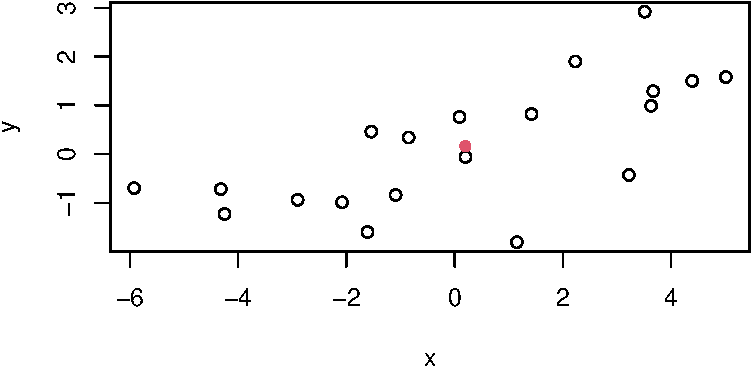
\includegraphics{CervantesAlvarez_Brian_HW1_ST557_files/figure-pdf/unnamed-chunk-3-1.pdf}

}

\end{figure}

\newpage{}

\hypertarget{part-c}{%
\subsection{Part C}\label{part-c}}

Find the sample covariance matrix.

\begin{Shaded}
\begin{Highlighting}[]
\CommentTok{\# Sample covariance matrix}
\NormalTok{sampCov }\OtherTok{\textless{}{-}} \FunctionTok{cov}\NormalTok{(ds)}

\NormalTok{sampCov}
\end{Highlighting}
\end{Shaded}

\begin{verbatim}
          X        Y
X 10.140227 2.852078
Y  2.852078 1.668133
\end{verbatim}

\newpage{}

\hypertarget{part-d}{%
\subsection{Part D}\label{part-d}}

Find the eigendecomposition (spectral decomposition) of the sample
covariance matrix using eigen().

\begin{Shaded}
\begin{Highlighting}[]
\NormalTok{sampEigenDecomp }\OtherTok{\textless{}{-}} \FunctionTok{eigen}\NormalTok{(sampCov)}

\NormalTok{sampEigenDecomp}
\end{Highlighting}
\end{Shaded}

\begin{verbatim}
eigen() decomposition
$values
[1] 11.0108859  0.7974741

$vectors
           [,1]       [,2]
[1,] -0.9564274  0.2919702
[2,] -0.2919702 -0.9564274
\end{verbatim}

\newpage{}

\hypertarget{part-e}{%
\subsection{Part E}\label{part-e}}

Add the eigenvector corresponding to the largest eigenvalue to the plot
as a vector from the sample mean using \texttt{lines()}. Be careful
here: if the first eigenvector is \((v_1, v_2)\) and the sample mean
vector is \((\bar{x}_1, \bar{x}_2)\), you want a line from
\((\bar{x}_1, \bar{x}_2)\) to \((\bar{x}_1 + v_1, \bar{x}_2 + v_2)\).''

\begin{Shaded}
\begin{Highlighting}[]
\CommentTok{\# Find the index of the largest eigenvalue}
\NormalTok{largestEigenvalue }\OtherTok{\textless{}{-}} \FunctionTok{which.max}\NormalTok{(sampEigenDecomp}\SpecialCharTok{$}\NormalTok{values)}
\CommentTok{\# Extract the eigenvector corresponding to the largest eigenvalue}
\NormalTok{largestEigenvector }\OtherTok{\textless{}{-}}\NormalTok{ sampEigenDecomp}\SpecialCharTok{$}\NormalTok{vectors[, largestEigenvalue]}

\CommentTok{\# Calculate the endpoints of the line segment}
\NormalTok{sampMeanX }\OtherTok{\textless{}{-}} \FunctionTok{mean}\NormalTok{(x)}
\NormalTok{sampMeanY }\OtherTok{\textless{}{-}} \FunctionTok{mean}\NormalTok{(y)}
\NormalTok{xend }\OtherTok{\textless{}{-}}\NormalTok{ sampMeanX }\SpecialCharTok{+}\NormalTok{ largestEigenvector[}\DecValTok{1}\NormalTok{]}
\NormalTok{yend }\OtherTok{\textless{}{-}}\NormalTok{ sampMeanY }\SpecialCharTok{+}\NormalTok{ largestEigenvector[}\DecValTok{2}\NormalTok{]}

\FunctionTok{plot}\NormalTok{(x,y)}
\CommentTok{\# Add the line segment to the plot}
\FunctionTok{lines}\NormalTok{(}\FunctionTok{c}\NormalTok{(sampMeanX, xend), }\FunctionTok{c}\NormalTok{(sampMeanY, yend), }\AttributeTok{col =} \StringTok{"seagreen4"}\NormalTok{, }\AttributeTok{lwd =} \DecValTok{3}\NormalTok{)}
\FunctionTok{points}\NormalTok{(sampMeanX, sampMeanY, }\AttributeTok{pch=}\DecValTok{16}\NormalTok{, }\AttributeTok{col=}\DecValTok{2}\NormalTok{)}
\end{Highlighting}
\end{Shaded}

\begin{figure}[H]

{\centering 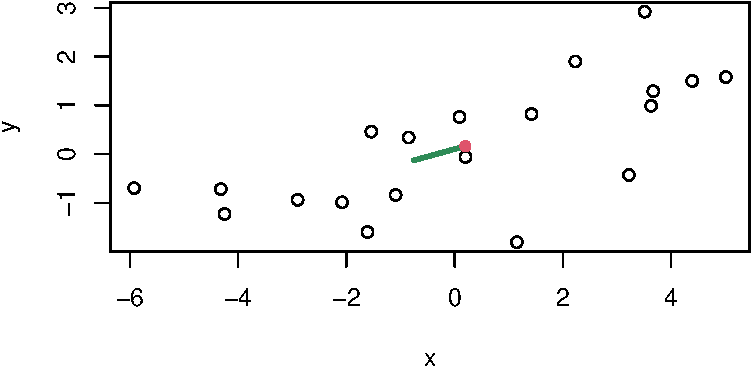
\includegraphics{CervantesAlvarez_Brian_HW1_ST557_files/figure-pdf/unnamed-chunk-6-1.pdf}

}

\end{figure}

\hypertarget{discussion-for-part-e}{%
\subsubsection{Discussion for Part E}\label{discussion-for-part-e}}

\textbf{Question: Describe how the direction of this eigenvector relates
to the cloud of data points}

The eigenvector follows the trend of the data points, which are showing
a positive increasing trend, and it culminates precisely at the location
of the sample means for X and Y.

\newpage{}

\hypertarget{question-2}{%
\section{Question 2}\label{question-2}}

\hypertarget{part-a-1}{%
\subsection{Part A}\label{part-a-1}}

\begin{Shaded}
\begin{Highlighting}[]
\NormalTok{ds }\OtherTok{\textless{}{-}} \FunctionTok{read.csv}\NormalTok{(}\StringTok{"CubitData.csv"}\NormalTok{)}
\FunctionTok{head}\NormalTok{(ds,}\DecValTok{5}\NormalTok{)}
\end{Highlighting}
\end{Shaded}

\begin{verbatim}
    height    cubit
1 70.98437 18.60823
2 70.82176 18.49283
3 70.62555 19.25116
4 71.31924 17.34156
5 71.35977 18.51334
\end{verbatim}

\begin{Shaded}
\begin{Highlighting}[]
\CommentTok{\# Calculate the sample mean vector}
\NormalTok{sampleMeanVec }\OtherTok{\textless{}{-}} \FunctionTok{colMeans}\NormalTok{(ds)}
\NormalTok{sampleMeanVec}
\end{Highlighting}
\end{Shaded}

\begin{verbatim}
  height    cubit 
67.08137 18.07067 
\end{verbatim}

\newpage{}

\hypertarget{part-b-1}{%
\subsection{Part B}\label{part-b-1}}

\begin{Shaded}
\begin{Highlighting}[]
\CommentTok{\# Calculate the sample covariance matrix!}
\NormalTok{sampleCovMatrix }\OtherTok{\textless{}{-}} \FunctionTok{cov}\NormalTok{(ds)}
\NormalTok{sampleCovMatrix}
\end{Highlighting}
\end{Shaded}

\begin{verbatim}
         height     cubit
height 5.604262 1.4548363
cubit  1.454836 0.8796708
\end{verbatim}

\newpage{}

\hypertarget{part-c-1}{%
\subsection{Part C}\label{part-c-1}}

\begin{Shaded}
\begin{Highlighting}[]
\CommentTok{\# Calculate the eigendecomposition using the covariance matrix, sampleCovMatrix}
\NormalTok{sampleEigenDecomp }\OtherTok{\textless{}{-}} \FunctionTok{eigen}\NormalTok{(sampleCovMatrix)}
\NormalTok{sampleEigenDecomp}
\end{Highlighting}
\end{Shaded}

\begin{verbatim}
eigen() decomposition
$values
[1] 6.0163114 0.4676216

$vectors
           [,1]       [,2]
[1,] -0.9621535  0.2725080
[2,] -0.2725080 -0.9621535
\end{verbatim}

\newpage{}

\hypertarget{part-d-1}{%
\subsection{Part D}\label{part-d-1}}

\begin{Shaded}
\begin{Highlighting}[]
\CommentTok{\# Find the index of the largest eigenvalue}
\NormalTok{largestEigenvalue }\OtherTok{\textless{}{-}} \FunctionTok{which.max}\NormalTok{(sampleEigenDecomp}\SpecialCharTok{$}\NormalTok{values)}
\CommentTok{\# Extract the eigenvector corresponding to the largest eigenvalue}
\NormalTok{largestEigenvector }\OtherTok{\textless{}{-}}\NormalTok{ sampleEigenDecomp}\SpecialCharTok{$}\NormalTok{vectors[, largestEigenvalue]}
\NormalTok{largestEigenvector}
\end{Highlighting}
\end{Shaded}

\begin{verbatim}
[1] -0.9621535 -0.2725080
\end{verbatim}

\newpage{}

\begin{Shaded}
\begin{Highlighting}[]
\CommentTok{\# Create the scatter plot}
\FunctionTok{plot}\NormalTok{(ds}\SpecialCharTok{$}\NormalTok{height, ds}\SpecialCharTok{$}\NormalTok{cubit)}

\CommentTok{\# Calculate each sample mean}
\NormalTok{meanCubit }\OtherTok{\textless{}{-}} \FunctionTok{mean}\NormalTok{(ds}\SpecialCharTok{$}\NormalTok{cubit)}
\NormalTok{meanHeight }\OtherTok{\textless{}{-}} \FunctionTok{mean}\NormalTok{(ds}\SpecialCharTok{$}\NormalTok{height)}

\CommentTok{\# Use Part D!}

\NormalTok{xend }\OtherTok{\textless{}{-}}\NormalTok{ meanHeight }\SpecialCharTok{+}\NormalTok{ largestEigenvector[}\DecValTok{1}\NormalTok{]}
\NormalTok{yend }\OtherTok{\textless{}{-}}\NormalTok{ meanCubit }\SpecialCharTok{+}\NormalTok{ largestEigenvector[}\DecValTok{2}\NormalTok{]}


\CommentTok{\# Plot the eigenvector as a line from the mean point}
\FunctionTok{lines}\NormalTok{(}\FunctionTok{c}\NormalTok{(meanHeight, xend), }\FunctionTok{c}\NormalTok{(meanCubit, yend), }\AttributeTok{col =} \StringTok{"seagreen4"}\NormalTok{, }\AttributeTok{lwd =} \DecValTok{3}\NormalTok{)}
\end{Highlighting}
\end{Shaded}

\begin{figure}[H]

{\centering 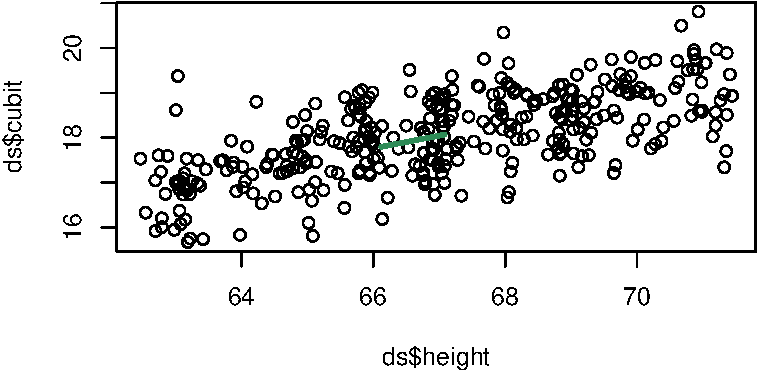
\includegraphics{CervantesAlvarez_Brian_HW1_ST557_files/figure-pdf/unnamed-chunk-11-1.pdf}

}

\end{figure}

\hypertarget{discussion-for-part-e-1}{%
\subsubsection{Discussion for Part E}\label{discussion-for-part-e-1}}

\textbf{Question: Describe how the direction of this eigenvector relates
to the cloud of data points}

The eigenvector for the height and cubit follows the trend of the data
points, which are showing a positive increasing trend. While not exactly
the same, it's similar to problem 1.

\newpage{}

\hypertarget{question-3}{%
\section{Question 3}\label{question-3}}

\hypertarget{part-a-2}{%
\subsection{Part A}\label{part-a-2}}

\begin{Shaded}
\begin{Highlighting}[]
\NormalTok{A }\OtherTok{\textless{}{-}} \FunctionTok{matrix}\NormalTok{(}\FunctionTok{c}\NormalTok{(}\FloatTok{5.125}\NormalTok{, }\FloatTok{3.875}\NormalTok{, }\FloatTok{2.125}\NormalTok{, }\SpecialCharTok{{-}}\FloatTok{1.125}\NormalTok{, }\DecValTok{0}\NormalTok{,}
              \FloatTok{3.875}\NormalTok{, }\FloatTok{5.125}\NormalTok{, }\SpecialCharTok{{-}}\FloatTok{1.125}\NormalTok{, }\FloatTok{2.125}\NormalTok{, }\DecValTok{0}\NormalTok{,}
              \FloatTok{2.125}\NormalTok{, }\SpecialCharTok{{-}}\FloatTok{1.125}\NormalTok{, }\FloatTok{5.125}\NormalTok{, }\FloatTok{3.875}\NormalTok{, }\DecValTok{0}\NormalTok{,}
              \SpecialCharTok{{-}}\FloatTok{1.125}\NormalTok{, }\FloatTok{2.125}\NormalTok{, }\FloatTok{3.875}\NormalTok{, }\FloatTok{5.125}\NormalTok{, }\DecValTok{0}\NormalTok{,}
              \DecValTok{0}\NormalTok{, }\DecValTok{0}\NormalTok{, }\DecValTok{0}\NormalTok{, }\DecValTok{0}\NormalTok{, }\SpecialCharTok{{-}}\DecValTok{3}\NormalTok{), }
            \AttributeTok{nrow =} \DecValTok{5}\NormalTok{, }
            \AttributeTok{byrow =} \ConstantTok{TRUE}\NormalTok{)}

\CommentTok{\# Calculate the eigendecomposition}
\NormalTok{eigenDecomposition }\OtherTok{\textless{}{-}} \FunctionTok{eigen}\NormalTok{(A)}
\NormalTok{eigenDecomposition}
\end{Highlighting}
\end{Shaded}

\begin{verbatim}
eigen() decomposition
$values
[1] 10.0  8.0  4.5 -2.0 -3.0

$vectors
     [,1] [,2] [,3] [,4] [,5]
[1,]  0.5  0.5 -0.5  0.5    0
[2,]  0.5  0.5  0.5 -0.5    0
[3,]  0.5 -0.5 -0.5 -0.5    0
[4,]  0.5 -0.5  0.5  0.5    0
[5,]  0.0  0.0  0.0  0.0    1
\end{verbatim}

\newpage{}

\hypertarget{part-b-2}{%
\subsection{Part B}\label{part-b-2}}

\begin{Shaded}
\begin{Highlighting}[]
\CommentTok{\# Grab the eigenvalues from the eigen decomposition}
\NormalTok{eigenvalues }\OtherTok{\textless{}{-}}\NormalTok{ eigenDecomposition}\SpecialCharTok{$}\NormalTok{values}
\CommentTok{\# Use the function "all" to check all eigenvalues to see if they\textquotesingle{}re positive definite}
\NormalTok{isPositiveDefinite }\OtherTok{\textless{}{-}} \FunctionTok{all}\NormalTok{(eigenvalues }\SpecialCharTok{\textgreater{}} \DecValTok{0}\NormalTok{)}
\NormalTok{isPositiveDefinite}
\end{Highlighting}
\end{Shaded}

\begin{verbatim}
[1] FALSE
\end{verbatim}

\begin{Shaded}
\begin{Highlighting}[]
\CommentTok{\# False! Now we need to find a vector x...}

\CommentTok{\# Get all eigenvector(s) that are negative}
\NormalTok{negVec }\OtherTok{\textless{}{-}}\NormalTok{ eigenDecomposition}\SpecialCharTok{$}\NormalTok{vectors[, }\FunctionTok{which}\NormalTok{(eigenvalues }\SpecialCharTok{\textless{}} \DecValTok{0}\NormalTok{)]}

\CommentTok{\# We need to normalize the eigenvector(s) using the equation }
\NormalTok{vecNorm }\OtherTok{\textless{}{-}}\NormalTok{ negVec }\SpecialCharTok{/} \FunctionTok{sqrt}\NormalTok{(}\FunctionTok{sum}\NormalTok{(negVec}\SpecialCharTok{\^{}}\DecValTok{2}\NormalTok{))}
\NormalTok{vecNorm}
\end{Highlighting}
\end{Shaded}

\begin{verbatim}
           [,1]      [,2]
[1,]  0.3535534 0.0000000
[2,] -0.3535534 0.0000000
[3,] -0.3535534 0.0000000
[4,]  0.3535534 0.0000000
[5,]  0.0000000 0.7071068
\end{verbatim}

\begin{Shaded}
\begin{Highlighting}[]
\NormalTok{result }\OtherTok{\textless{}{-}} \FunctionTok{t}\NormalTok{(vecNorm) }\SpecialCharTok{\%*\%}\NormalTok{ A }\SpecialCharTok{\%*\%}\NormalTok{ vecNorm}
\NormalTok{result}
\end{Highlighting}
\end{Shaded}

\begin{verbatim}
     [,1] [,2]
[1,]   -1  0.0
[2,]    0 -1.5
\end{verbatim}

We end of getting a vector
\(x = \begin{bmatrix} 0.3535534 \\ -0.3535534 \\ -0.3535534 \\ 0.3535534 \\ 0 \end{bmatrix}\)
for which \(x^T A x < 0\), confirming that \(A\) is not positive
definite.

\newpage{}

\hypertarget{part-c-2}{%
\subsection{Part C}\label{part-c-2}}

The matrix-vector multiplication \(Ax\), where \(x = 4v_1 + 2v_5\), can
be expressed symbolically as:

\[Ax = 4\lambda_1 v_1 + 2\lambda_5 v_5\]

In this expression, \(\lambda_1\) and \(\lambda_5\) are the eigenvalues
corresponding to \(v_1\) and \(v_5\), respectively. If we want to
calculate it, we could plug in the eigenvalues and solve.

\newpage{}

\hypertarget{question-4}{%
\section{Question 4}\label{question-4}}

\hypertarget{part-a-3}{%
\subsection{Part A}\label{part-a-3}}

\begin{Shaded}
\begin{Highlighting}[]
\CommentTok{\# Read the data from the CSV file}
\NormalTok{ds }\OtherTok{\textless{}{-}} \FunctionTok{read.csv}\NormalTok{(}\StringTok{"IrisData.csv"}\NormalTok{)}
\FunctionTok{names}\NormalTok{(ds)}
\end{Highlighting}
\end{Shaded}

\begin{verbatim}
[1] "Sepal.Length" "Sepal.Width"  "Petal.Length" "Petal.Width"  "Type"        
\end{verbatim}

\begin{Shaded}
\begin{Highlighting}[]
\CommentTok{\# Calculate the sample mean vector for all variables}
\NormalTok{meanVec }\OtherTok{\textless{}{-}} \FunctionTok{colMeans}\NormalTok{(ds[,])}
\NormalTok{meanVec}
\end{Highlighting}
\end{Shaded}

\begin{verbatim}
Sepal.Length  Sepal.Width Petal.Length  Petal.Width         Type 
    5.843333     3.057333     3.758000     1.199333     2.000000 
\end{verbatim}

\begin{Shaded}
\begin{Highlighting}[]
\FunctionTok{print}\NormalTok{(ds}\SpecialCharTok{$}\NormalTok{Type)}
\end{Highlighting}
\end{Shaded}

\begin{verbatim}
  [1] 1 1 1 1 1 1 1 1 1 1 1 1 1 1 1 1 1 1 1 1 1 1 1 1 1 1 1 1 1 1 1 1 1 1 1 1 1
 [38] 1 1 1 1 1 1 1 1 1 1 1 1 1 2 2 2 2 2 2 2 2 2 2 2 2 2 2 2 2 2 2 2 2 2 2 2 2
 [75] 2 2 2 2 2 2 2 2 2 2 2 2 2 2 2 2 2 2 2 2 2 2 2 2 2 2 3 3 3 3 3 3 3 3 3 3 3
[112] 3 3 3 3 3 3 3 3 3 3 3 3 3 3 3 3 3 3 3 3 3 3 3 3 3 3 3 3 3 3 3 3 3 3 3 3 3
[149] 3 3
\end{verbatim}

\newpage{}

\hypertarget{part-b-3}{%
\subsection{Part B}\label{part-b-3}}

\begin{Shaded}
\begin{Highlighting}[]
\CommentTok{\# Calculate the sample mean vector for each species}
\NormalTok{species1MeanVec }\OtherTok{\textless{}{-}} \FunctionTok{colMeans}\NormalTok{(ds[ds}\SpecialCharTok{$}\NormalTok{type }\SpecialCharTok{==} \DecValTok{1}\NormalTok{, }\DecValTok{1}\SpecialCharTok{:}\DecValTok{4}\NormalTok{])}
\NormalTok{species2MeanVec }\OtherTok{\textless{}{-}} \FunctionTok{colMeans}\NormalTok{(ds[ds}\SpecialCharTok{$}\NormalTok{type }\SpecialCharTok{==} \DecValTok{2}\NormalTok{, }\DecValTok{1}\SpecialCharTok{:}\DecValTok{4}\NormalTok{])}
\NormalTok{species3MeanVec }\OtherTok{\textless{}{-}} \FunctionTok{colMeans}\NormalTok{(ds[ds}\SpecialCharTok{$}\NormalTok{type }\SpecialCharTok{==} \DecValTok{3}\NormalTok{, }\DecValTok{1}\SpecialCharTok{:}\DecValTok{4}\NormalTok{])}
\end{Highlighting}
\end{Shaded}

\newpage{}

\hypertarget{part-c-3}{%
\subsection{Part C}\label{part-c-3}}

\begin{Shaded}
\begin{Highlighting}[]
\CommentTok{\# Calculate the sample correlation matrix for all variables}
\NormalTok{corMatrix }\OtherTok{\textless{}{-}} \FunctionTok{cor}\NormalTok{(ds[,])}
\NormalTok{corMatrix}
\end{Highlighting}
\end{Shaded}

\begin{verbatim}
             Sepal.Length Sepal.Width Petal.Length Petal.Width       Type
Sepal.Length    1.0000000  -0.1175698    0.8717538   0.8179411  0.7825612
Sepal.Width    -0.1175698   1.0000000   -0.4284401  -0.3661259 -0.4266576
Petal.Length    0.8717538  -0.4284401    1.0000000   0.9628654  0.9490347
Petal.Width     0.8179411  -0.3661259    0.9628654   1.0000000  0.9565473
Type            0.7825612  -0.4266576    0.9490347   0.9565473  1.0000000
\end{verbatim}

\newpage{}

\hypertarget{part-d-2}{%
\subsection{Part D}\label{part-d-2}}

\begin{Shaded}
\begin{Highlighting}[]
\CommentTok{\# Calculate individual correlation matrices for each species}
\NormalTok{species1CorMatrix }\OtherTok{\textless{}{-}} \FunctionTok{cor}\NormalTok{(ds[ds}\SpecialCharTok{$}\NormalTok{type }\SpecialCharTok{==} \DecValTok{1}\NormalTok{, }\DecValTok{1}\SpecialCharTok{:}\DecValTok{4}\NormalTok{])}
\NormalTok{species2CorMatrix }\OtherTok{\textless{}{-}} \FunctionTok{cor}\NormalTok{(ds[ds}\SpecialCharTok{$}\NormalTok{type }\SpecialCharTok{==} \DecValTok{2}\NormalTok{, }\DecValTok{1}\SpecialCharTok{:}\DecValTok{4}\NormalTok{])}
\NormalTok{species3CorMatrix }\OtherTok{\textless{}{-}} \FunctionTok{cor}\NormalTok{(ds[ds}\SpecialCharTok{$}\NormalTok{type }\SpecialCharTok{==} \DecValTok{3}\NormalTok{, }\DecValTok{1}\SpecialCharTok{:}\DecValTok{4}\NormalTok{])}
\end{Highlighting}
\end{Shaded}

\newpage{}

\hypertarget{part-e-1}{%
\subsection{Part E}\label{part-e-1}}

\begin{Shaded}
\begin{Highlighting}[]
\FunctionTok{library}\NormalTok{(ggplot2)}

\FunctionTok{pairs}\NormalTok{(ds[, }\DecValTok{1}\SpecialCharTok{:}\DecValTok{4}\NormalTok{], }
      \AttributeTok{main =} \StringTok{"Pairs Plot for Iris Dataset"}\NormalTok{,}
      \AttributeTok{pch =} \DecValTok{21}\NormalTok{, }\AttributeTok{col =} \FunctionTok{as.numeric}\NormalTok{(ds}\SpecialCharTok{$}\NormalTok{Type), }
      \AttributeTok{labels =} \FunctionTok{colnames}\NormalTok{(ds)[}\DecValTok{1}\SpecialCharTok{:}\DecValTok{4}\NormalTok{],}
      \AttributeTok{lower.panel =}\NormalTok{ panel.smooth,}
\NormalTok{)}
\end{Highlighting}
\end{Shaded}

\begin{figure}[H]

{\centering 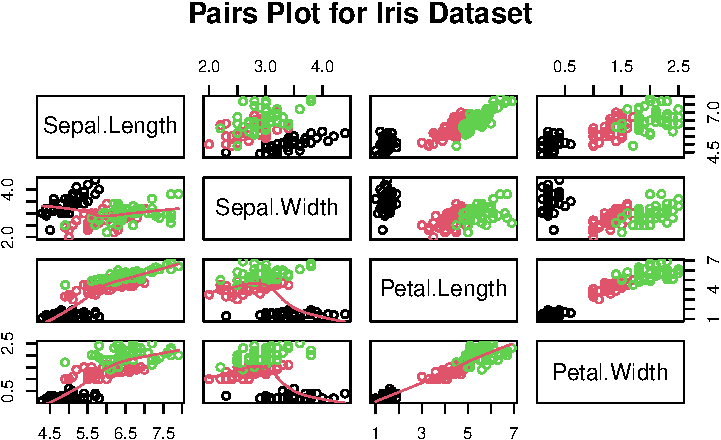
\includegraphics{CervantesAlvarez_Brian_HW1_ST557_files/figure-pdf/unnamed-chunk-18-1.pdf}

}

\end{figure}

You can totally spot some noticeable differences among these flowers.
When it comes to telling them apart, Petal Width seems to be the way to
go, thanks to their clear clustering that lets you easily identify the
species. And if you look at Petal Length and Petal Width, it's pretty
apparent that they both follow a nice linear pattern in their
clustering, making it even easier to tell them apart based on these
features.

\newpage{}

\hypertarget{question-5}{%
\section{Question 5}\label{question-5}}



\end{document}
